\documentclass{beamer}
\usetheme{Boadilla}
\usepackage{tikz}
 \usepackage[english]{babel}
 \usepackage{amsmath}
 \usepackage{amssymb}
 \usepackage{amsthm}
 \usepackage{animate}
 \usepackage{mathtools} 
 \usepackage[utf8]{inputenc}
 \usepackage{dsfont}
 \usetikzlibrary{patterns}
 \usepackage{mathrsfs}
 \usepackage{bbold}
 \usepackage{tcolorbox}
 \usepackage{txfonts}
\usetikzlibrary{mindmap,trees,shadows}
\usepackage{caption}
\usepackage{tabularx}
\usepackage{booktabs}
\usepackage{apacite}
\usepackage{listings}
\captionsetup[figure]{font=scriptsize}
\newcommand{\MYhref}[3][blue]{\href{#2}{\color{#1}{#3}}}%
\usepackage{hyperref} 
            \hypersetup{backref=true,       
                    pagebackref=true,               
                    hyperindex=true,                
                    colorlinks=true,                
                    breaklinks=true,                
                    urlcolor= blue,                
                    linkcolor= blue,                
                    bookmarks=true,                 
                    bookmarksopen=false,
                    citecolor=blue,
                    linkcolor=blue,
                    filecolor=blue,
                    citecolor=blue,
                    linkbordercolor=blue
}

\definecolor{background}{RGB}{39, 40, 34}
\definecolor{string}{RGB}{230, 219, 116}
\definecolor{comment}{RGB}{117, 113, 94}
\definecolor{normal}{RGB}{248, 248, 242}
\definecolor{identifier}{RGB}{166, 226, 46}

\lstset{
  language = SQL,  % choose the language of the code
  linewidth = 12cm,
  numbers = left, % where to put the line-numbers
  stepnumber=1,  % the step between two line-numbers.
  numbersep=5pt, % how far the line-numbers are from the code
  numberstyle=\tiny\color{black}\ttfamily,
  backgroundcolor=\color{background}, % choose the background color. You must add \usepackage{color}
  showspaces=false, % show spaces adding particular underscores
  showstringspaces=false,             % underline spaces within strings
  showtabs=false, % show tabs within strings adding particular underscores
  tabsize=4,                          % sets default tabsize to 2 spaces
  captionpos=b,                       % sets the caption-position to bottom
  breaklines=true,                    % sets automatic line breaking
  breakatwhitespace=true, % sets if automatic breaks should only happen at whitespace
  title=\lstname,  % show the filename of files included with \lstinputlisting;
  basicstyle=\color{normal}\ttfamily,     % sets font style for the code
  keywordstyle=\color{magenta}\ttfamily,  % sets color for keywords
  stringstyle=\color{string}\ttfamily,    % sets color for strings
  commentstyle=\color{comment}\ttfamily,  % sets color for comments
  emph={format_string, eff_ana_bf, permute, eff_ana_btr},
  emphstyle=\color{identifier}\ttfamily,
  belowskip=-0.5cm
}

\newcommand{\pic}[1]{%
    \includegraphics[width=4cm]{#1}
}

\title[High Dimensional Models] % (optional, only for long titles)
{High Dimensional Models}
\subtitle{Time-Varying Graphical Lasso}
\author[Andrew Boomer \& Jacob Pichelmann] % (optional, for multiple authors)
{Andrew Boomer \& Jacob Pichelmann}
\institute []
{Toulouse School of Economics \\ M2 EEE}


\usepackage{graphicx}
\usepackage{grffile}

\date{\today}

\graphicspath{
    {.} % document root dir
    {./Output/}
    {./Report/}
}

\begin{document}

\frame{\titlepage}
    

\begin{frame}{Overview}
	\begin{enumerate}
		\item Introduction to Graphical Models
		\begin{itemize}
			\item Important Properties
			\item Interpretation
		\end{itemize}
		\item Gaussian Graphical Model
		\item Time Varying Graphical Lasso (TGLV)
		\begin{itemize}
			\item Altered Optimisation Problem
			\item ADMM
		\end{itemize}
		\item Practical Application of TGVL
		\begin{itemize}
			\item Comparison to Static Graphical Lasso
			\item Changing the penalty function
		\end{itemize}
		\end{enumerate}
\end{frame}

\begin{frame}{Graphical Models}
\begin{itemize}
	\item Graphical models offer a way to encode conditional dependencies between $p$ random variables $X_1, \cdots, X_p$ by a graph $g$
	\item A graph consists of a vertex set $V = \{1,2, \cdots, p\}$ and an edge set $E \subset V \times V$
	\item We focus on undirected graphical models, i.e. no distinction between an edge $(s, t) \in E$ and the edge $(t,s)$.
\end{itemize}
Consider the following example:
\begin{figure}
	\caption{Undirected Graphical Model}
	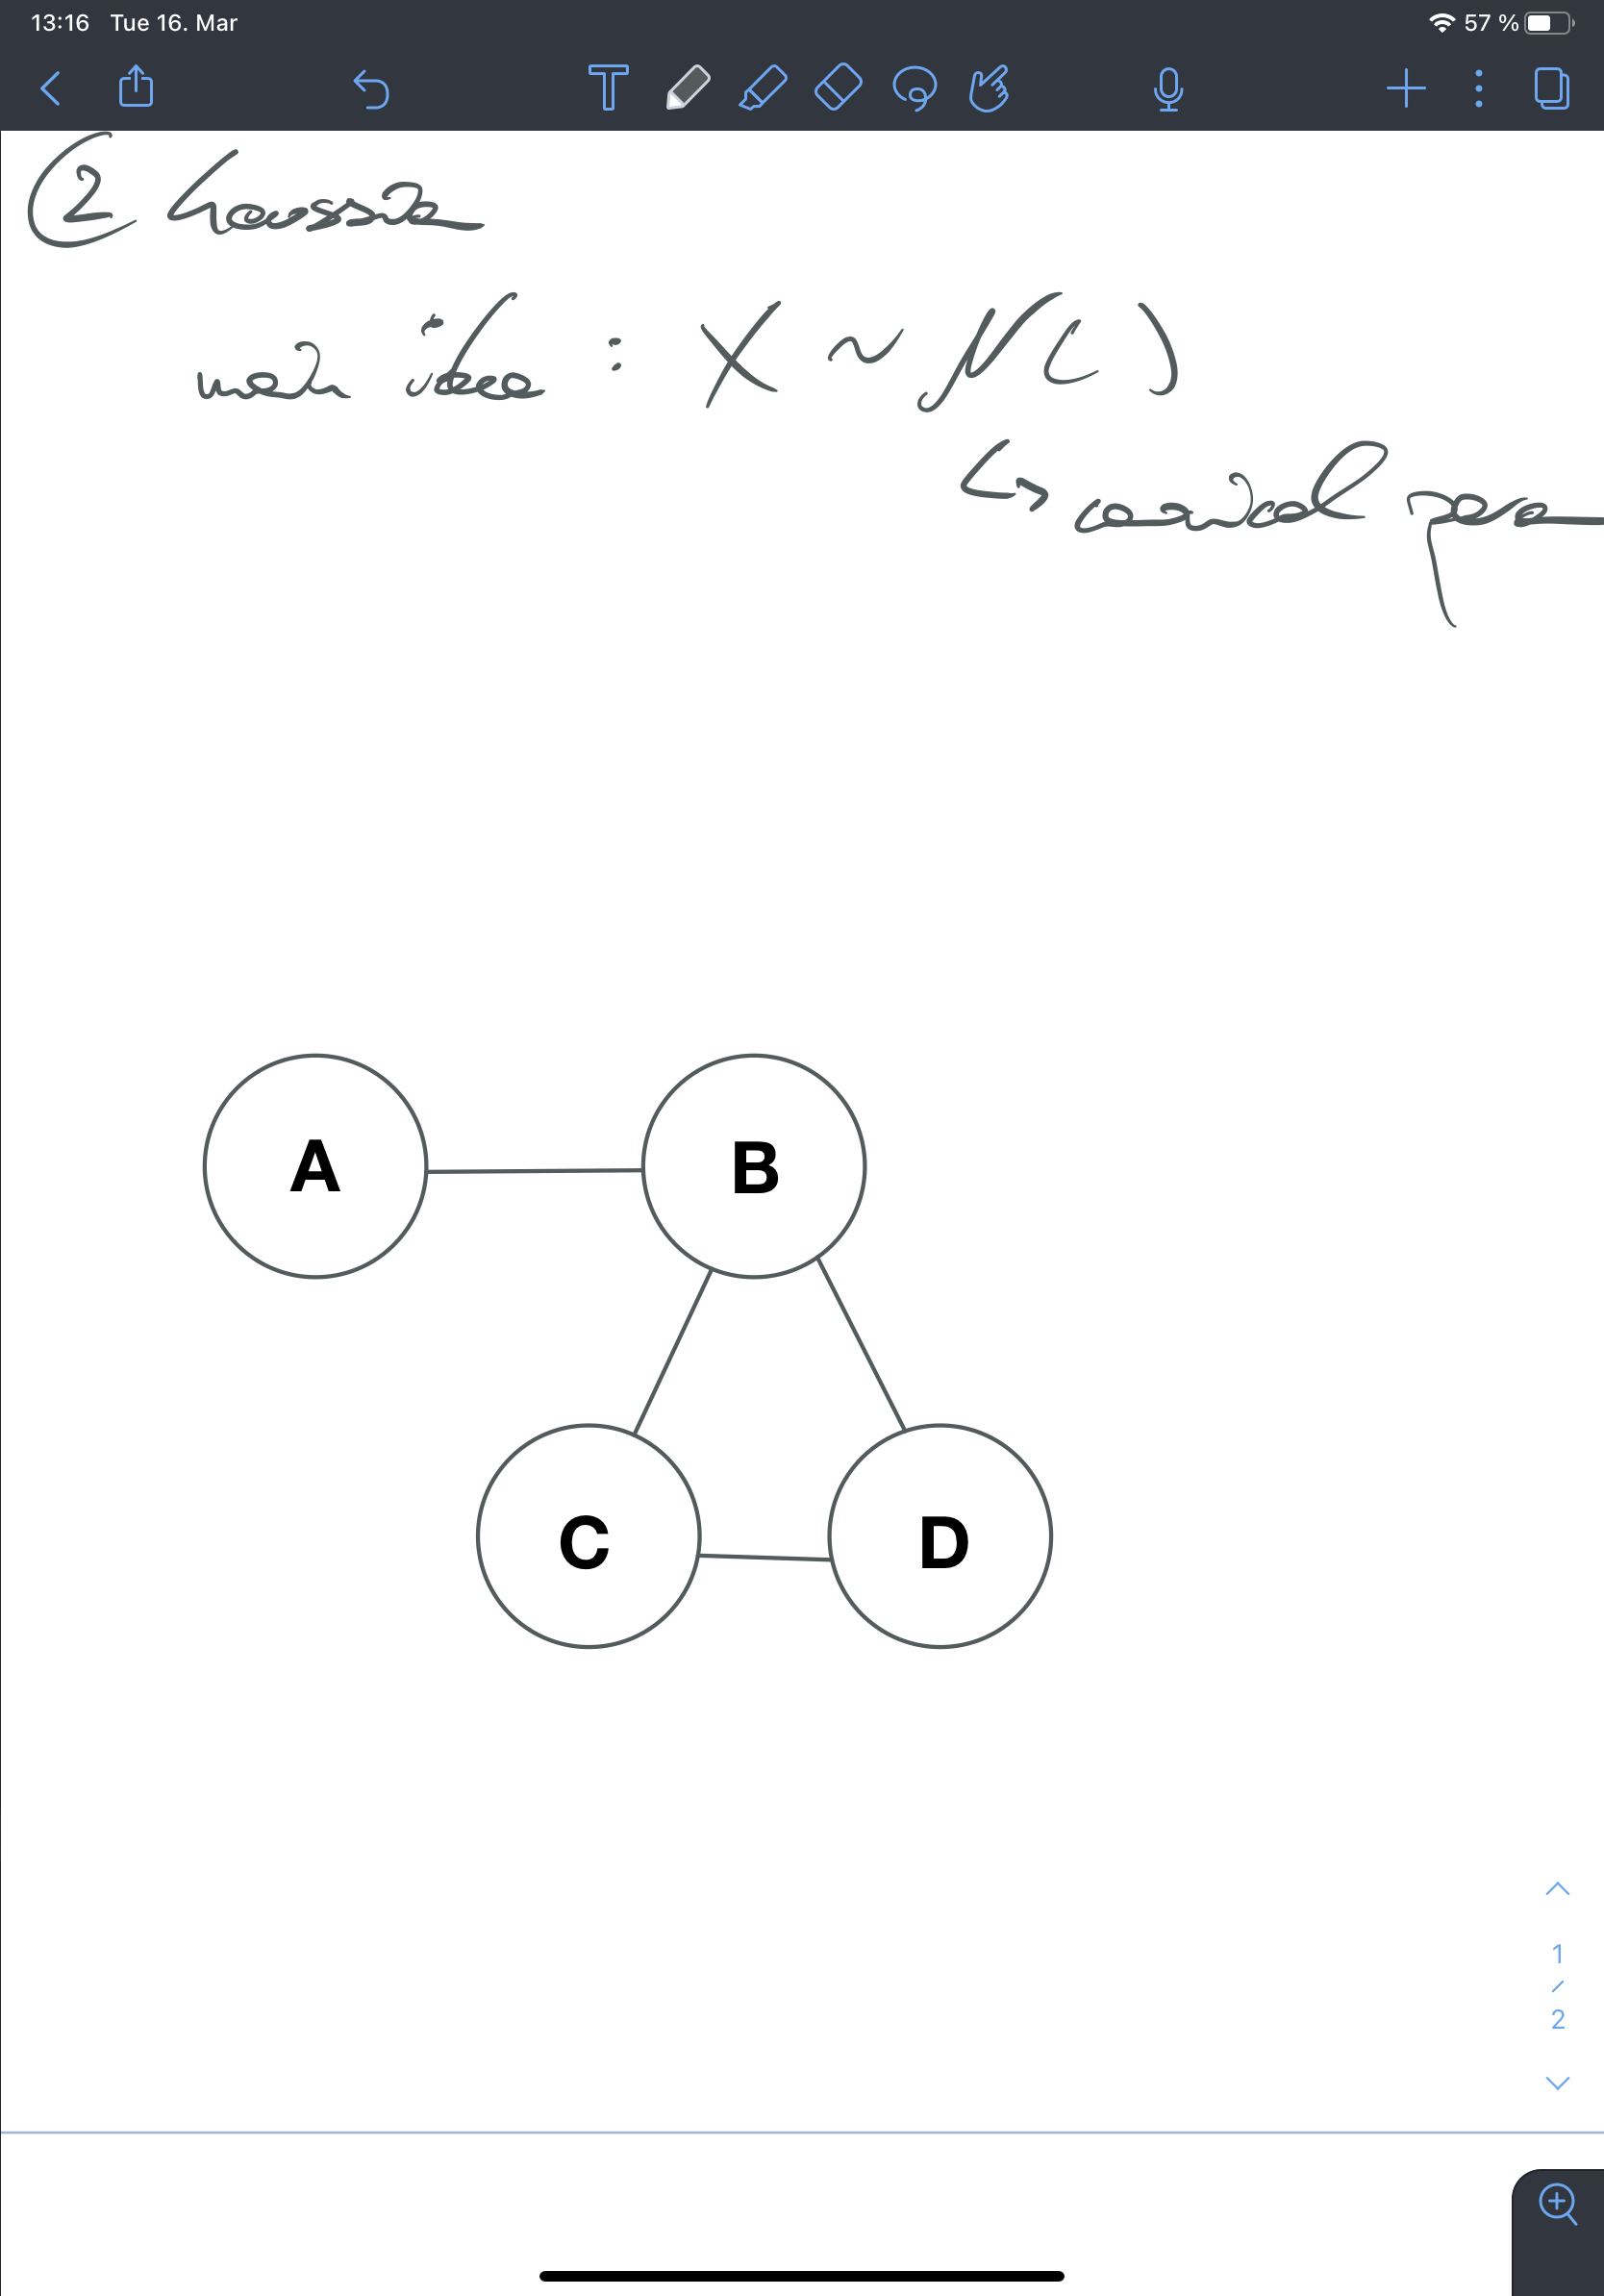
\includegraphics[trim={2cm 2cm 10cm 38cm}, clip, width = 7cm]{graphs/IMG_0091}
\end{figure}
\end{frame}

\begin{frame}{Factorization Property}
A graph clique $C \subseteq V$ is a fully-connected subset of the vertex set, i.e. $(s,t) \in E \forall s,t \in C$. \cite{hastie2015statistical}
\begin{align*}
	\mathbb{P}(A, B, C, D) &\propto \phi(A,B) \phi(B, C, D) \\
	P(X) &= \frac{1}{Z} \prod_{c \in C} \phi c (x_c)
\end{align*}
\begin{figure}
	\caption{Maximal Cliques}
	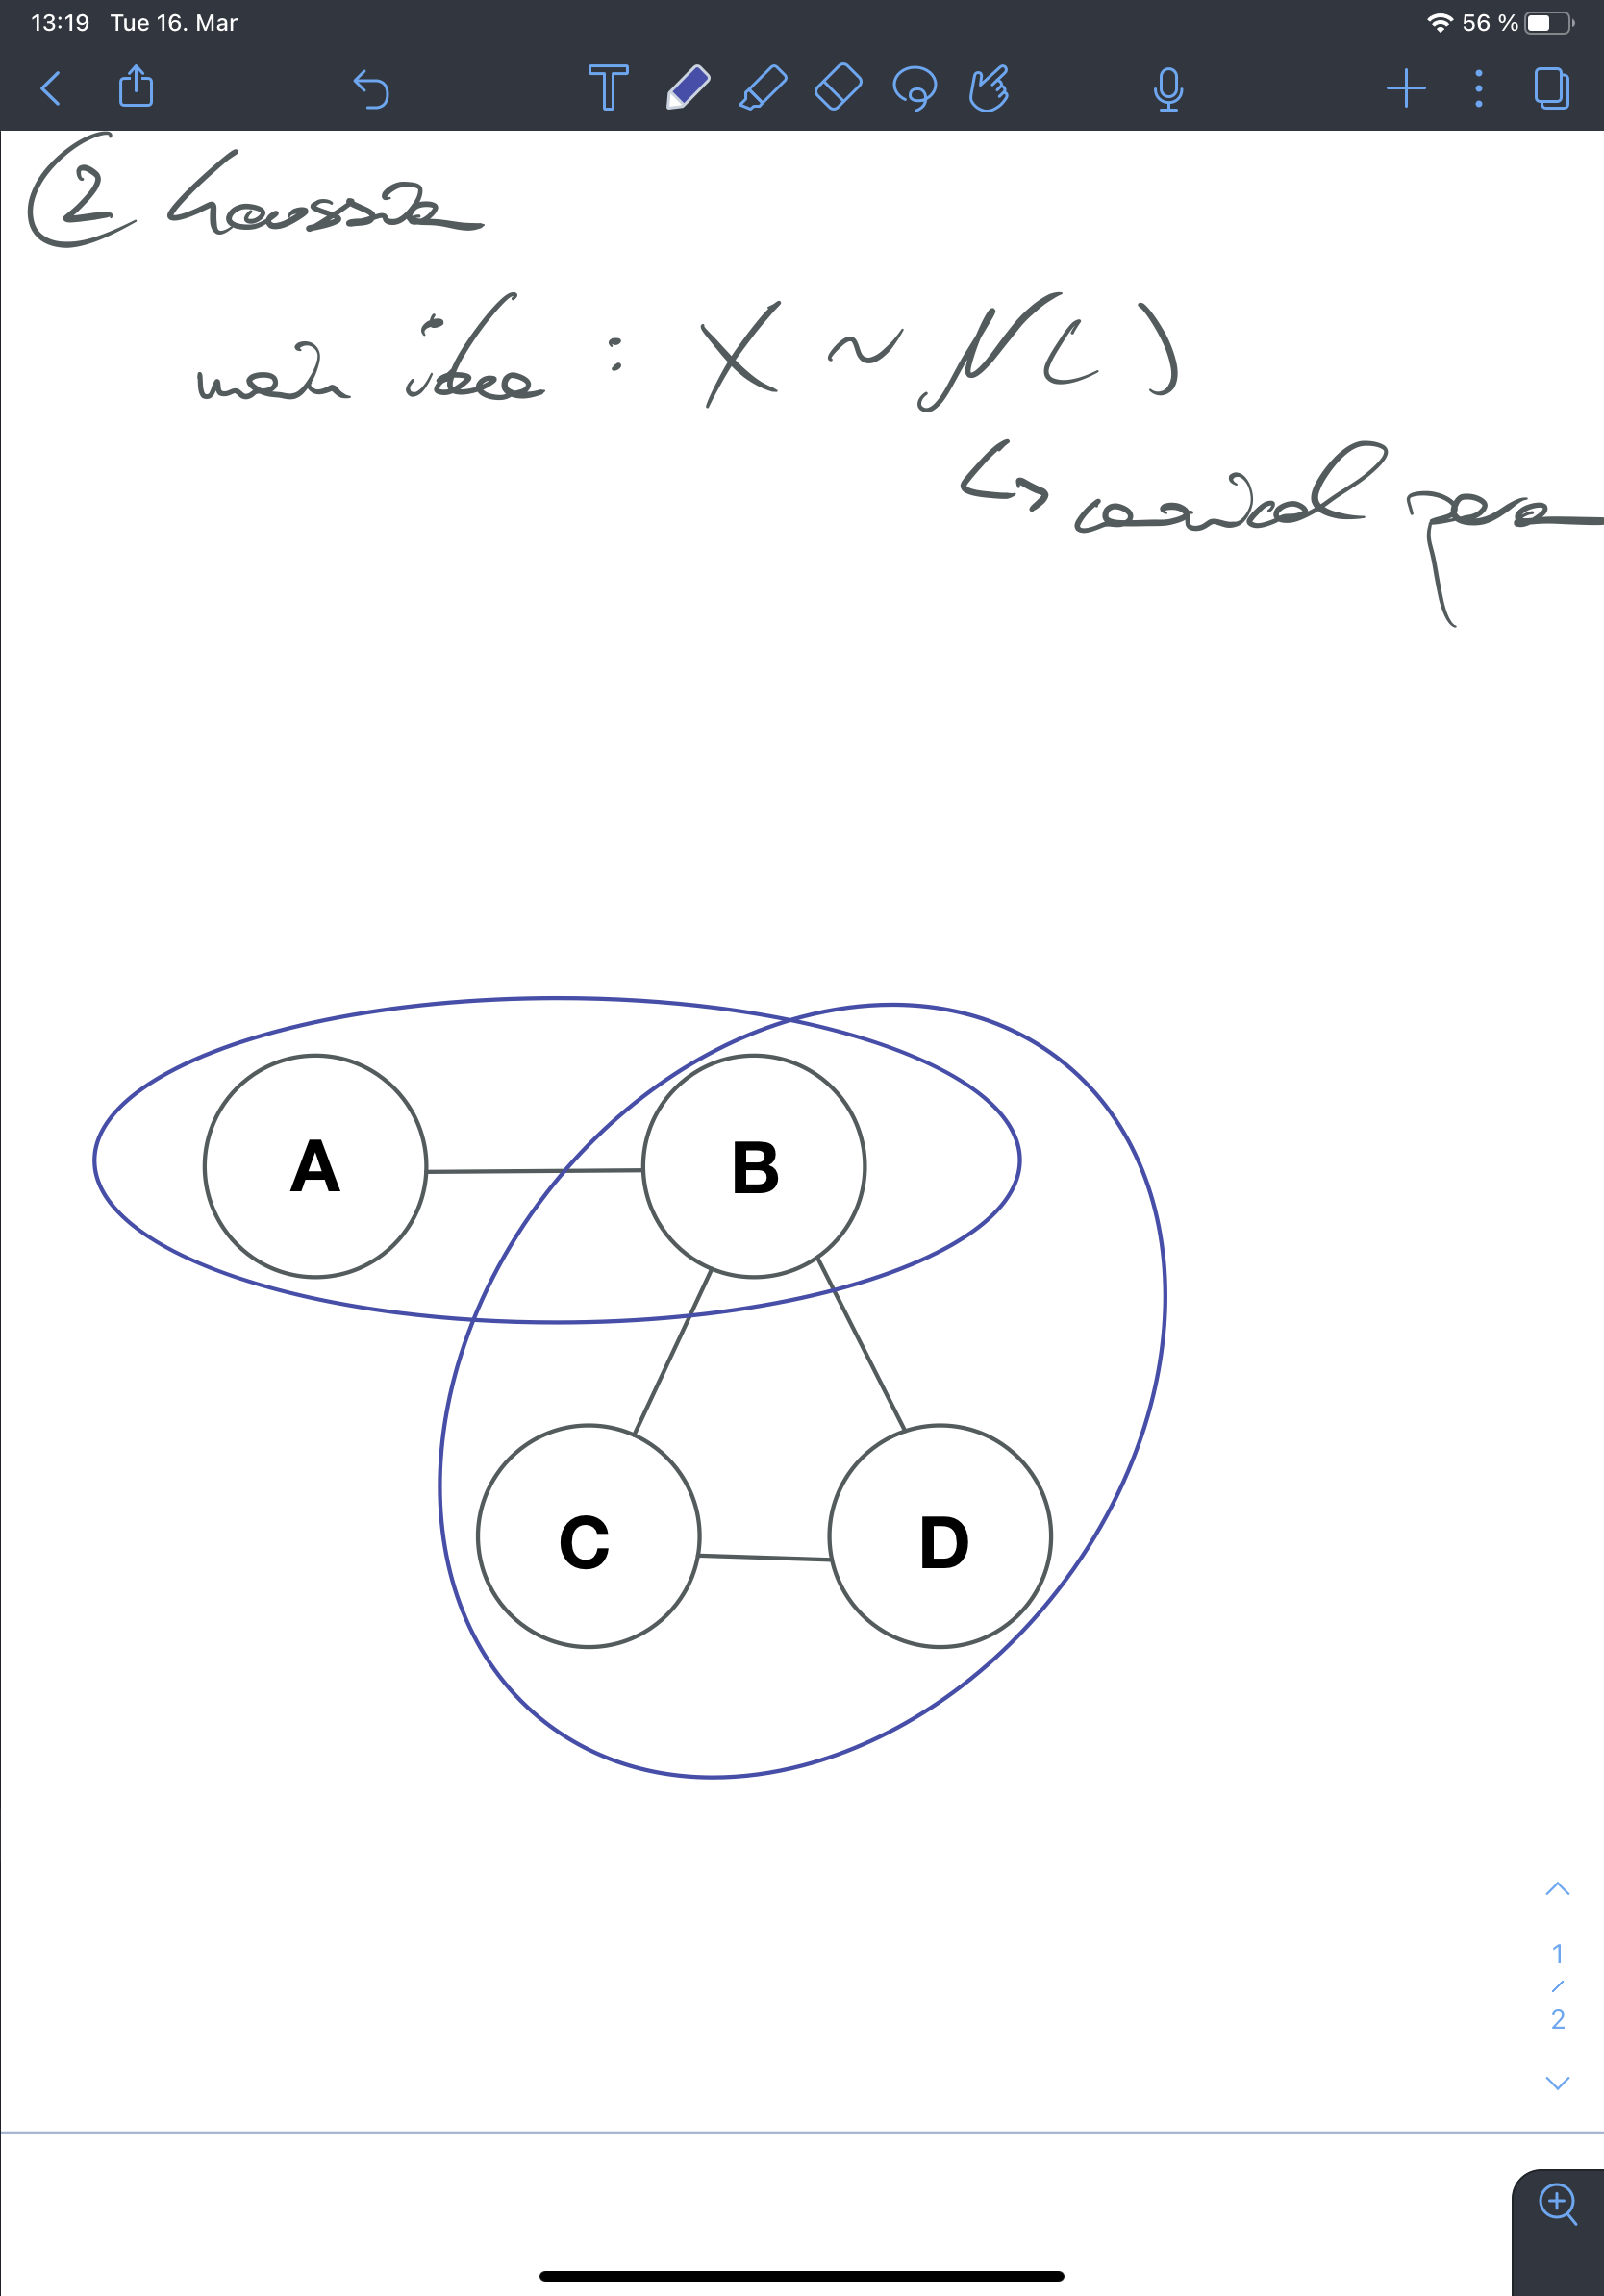
\includegraphics[trim={2cm 18cm 10cm 35cm}, clip, width = 6.5cm]{graphs/IMG_0093}
\end{figure}
\end{frame}

\begin{frame}{Markov Property}
Any two subsets $S$ and $T$ are conditionally independent given a separating subset $Y$. A random vector $X$ is Markov with respect to $g$ if
\begin{align*}
	X_S \Perp X_T | X_Y \text{ for all cut sets } S \subset V.
\end{align*}
\begin{figure}
	\caption{Separating Set: $\{ B, C\}$}
	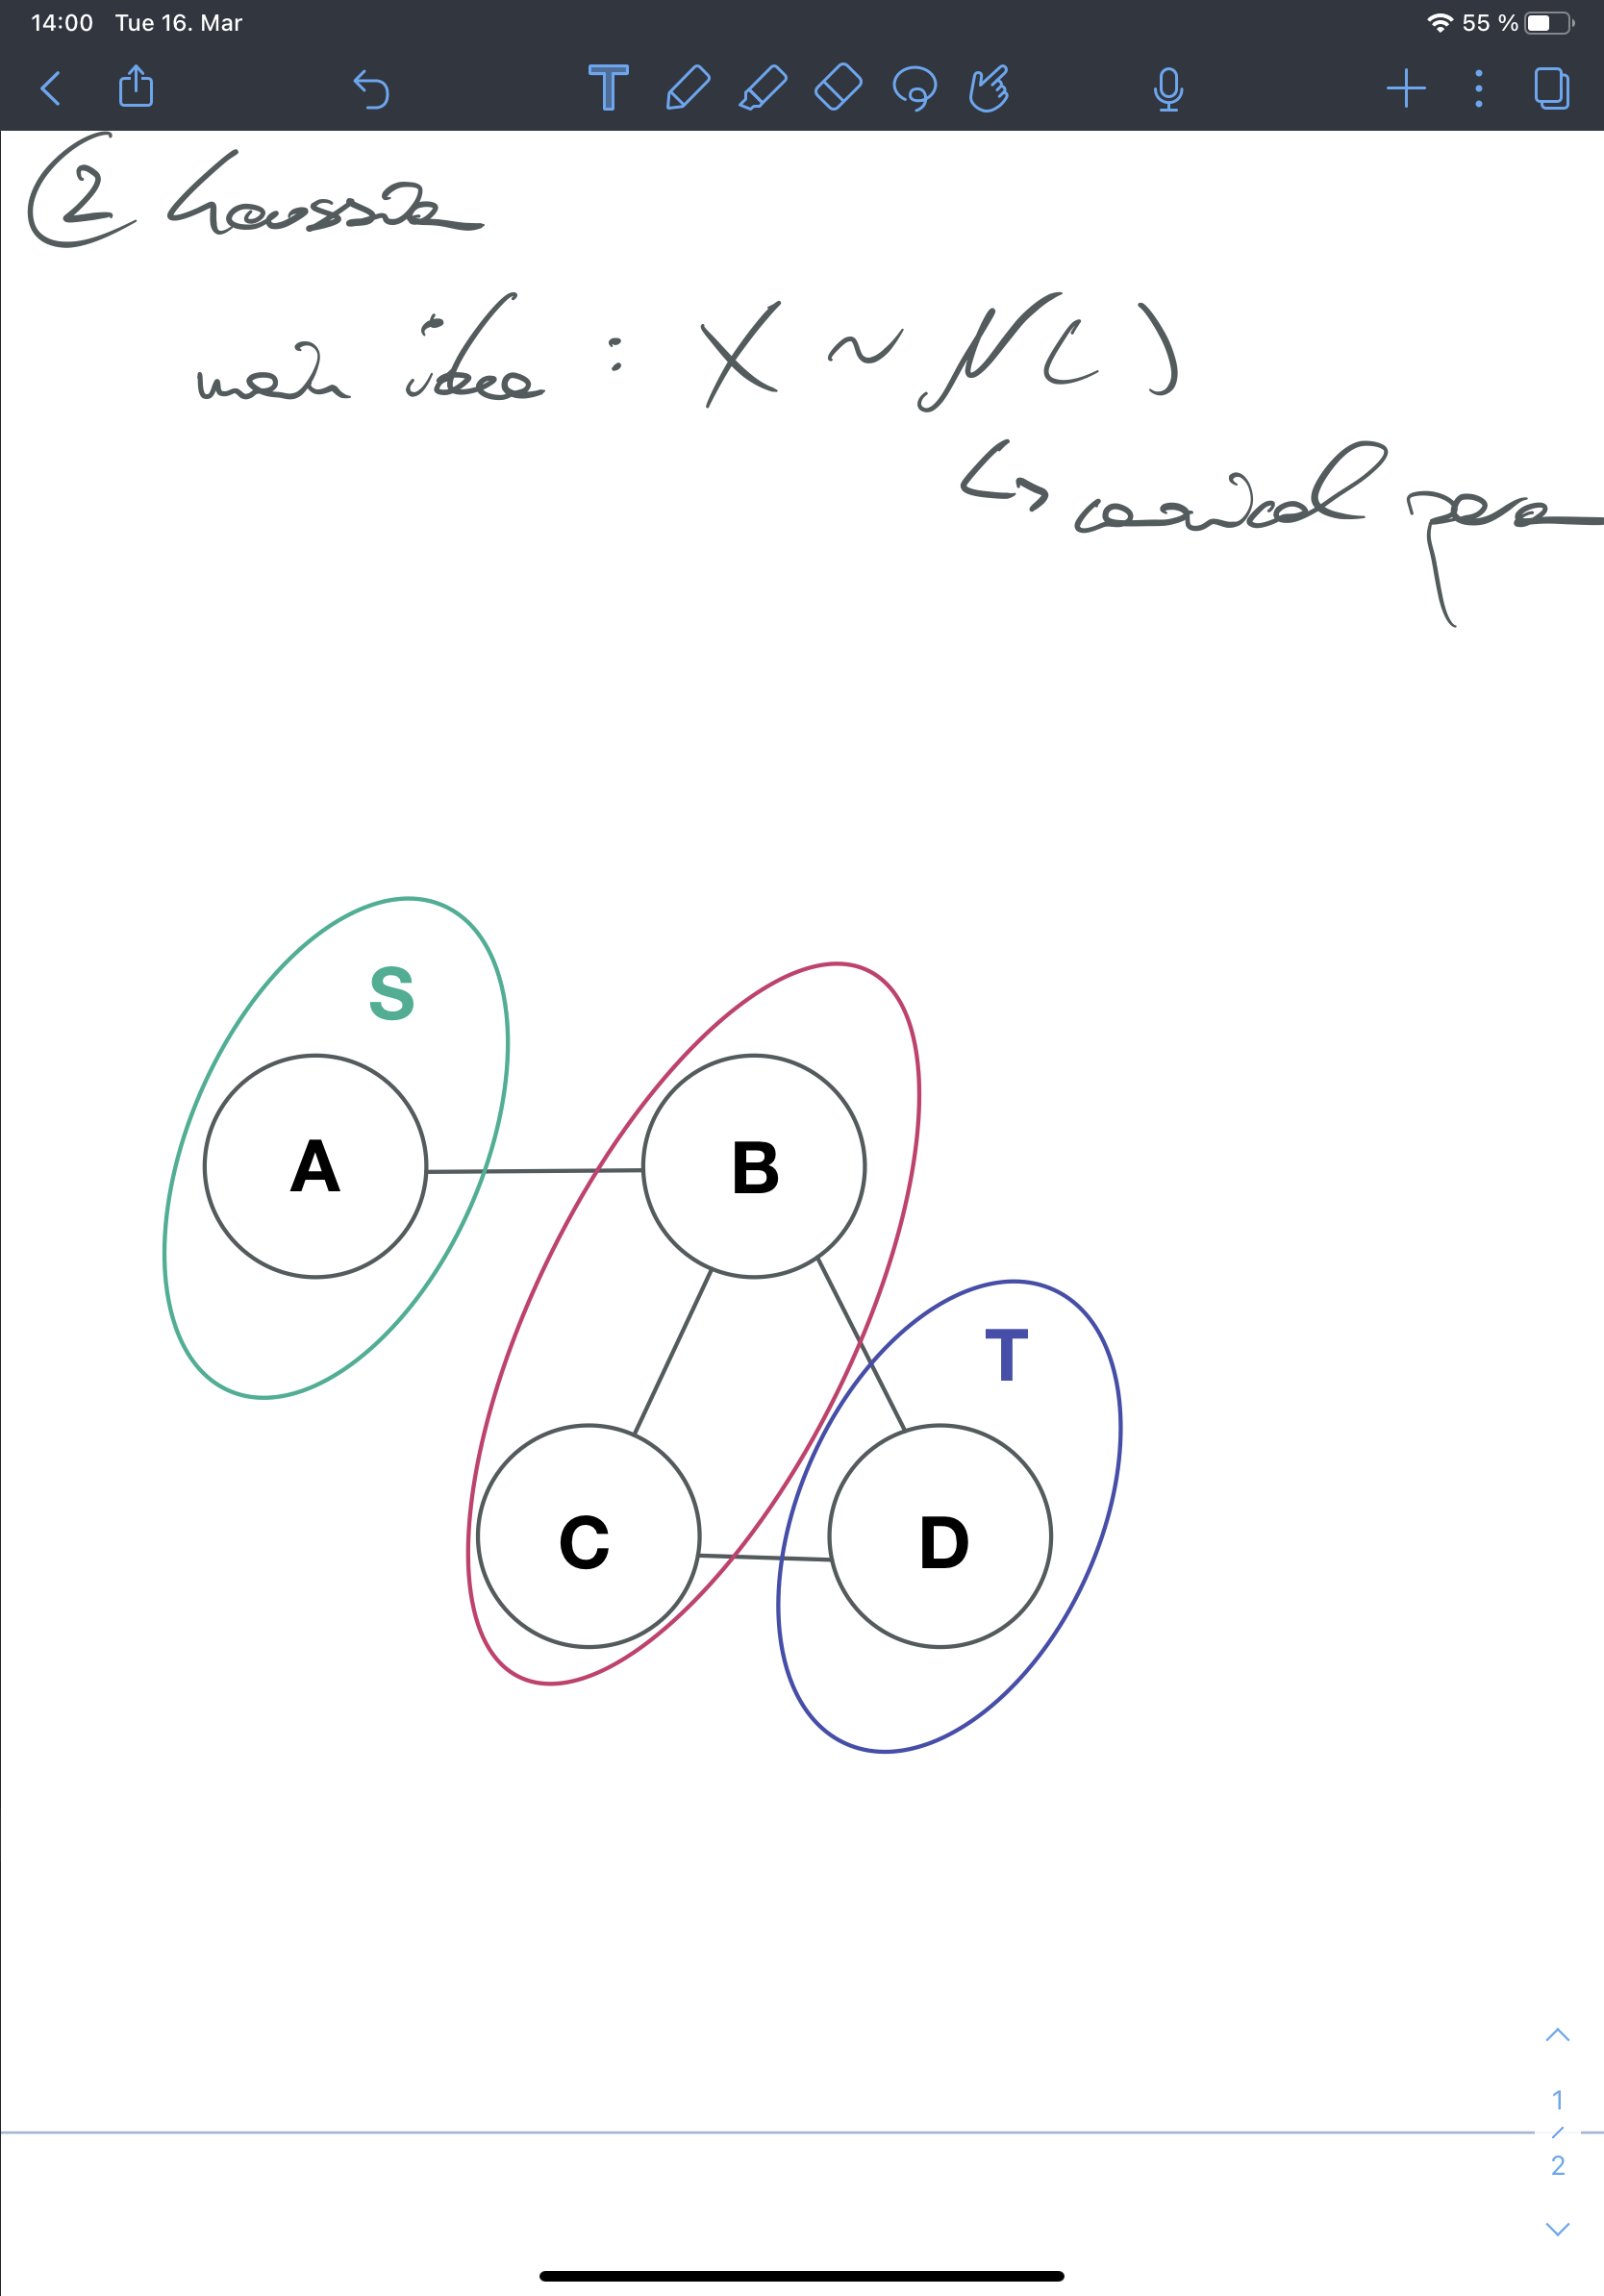
\includegraphics[trim={2cm 2cm 10cm 32cm}, clip, width = 7cm]{graphs/IMG_0094}
\end{figure}
\end{frame}

\begin{frame}{Equivalence of Properties}
\begin{itemize}
	\item Hammersley-Clifford theorem: \begin{center}
		\textit{For any strictly positive distribution the distribution of $X$ factorizes according to the graph $g$ if and only if the random vector X is Markov with respect to the graph.} \cite{hastie2015statistical}
	\end{center}
\end{itemize}
\end{frame}


\begin{frame}{Gaussian Graphical Model}
\begin{center}
		\begin{tcolorbox}[width = 4.5in, boxsep = 0pt,
			left = 2pt, right = 2pt, top = 2pt]
			\begin{align*}
			X \sim \mathcal{N}(\mu, \Sigma)
			\end{align*}
			If $\Sigma$ is positive definite, distribution has density on $\mathbb{R}^{p}$
\begin{align*}
	f(x \mid \mu, \Sigma)=(2 \pi)^{-p / 2}(\operatorname{det} \Theta)^{1 / 2} e^{-(x-\mu)^{T} \Theta(x-\mu) / 2}
\end{align*}
where $\Theta=\Sigma^{-1}$ is the Precision matrix of the distribution.
		\end{tcolorbox}	
\end{center}

Empirical covariance $S = \frac{1}{n-1} \sum_{i=1}^{n}\left(x_{i}-\mu\right)\left(x_{i}-\mu\right)'$

\end{frame}

\begin{frame}{Gaussian Graphical Model}
	A multivariate Gaussian distribution can be represented by a Markov random field, i.e. an undirected graph $g = (V, E)$ with
	\begin{itemize}
		\item the vertex set $V = \{1, \cdots, p \}$ corresponding to the random variables and
		\item the edge set $E = \left\{(i, j) \in V \mid i \neq j, \Theta_{i j} \neq 0\right\}$
	\end{itemize}
	\begin{figure}
		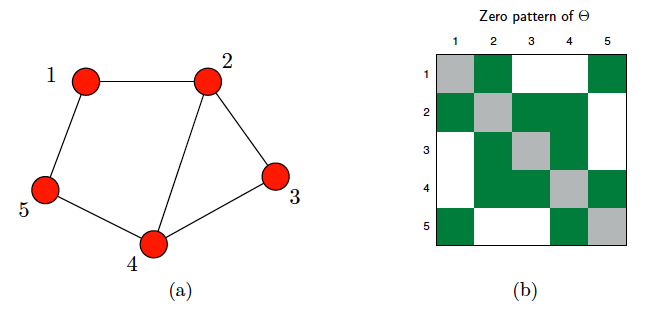
\includegraphics[trim={0 2cm 0 0}, clip,width = 8cm]{IntroGraphMat}
	\end{figure}
\end{frame}


\begin{frame}{Estimating the graph structure $\Leftrightarrow \Theta$}
  \begin{itemize}
      \item Suppose $X$ denotes samples from a multivariate Gaussian distribution with $\mu = 0$ and precision matrix $\Theta \in \mathbb{R}^{p \times p}$
    \item We can write the log-likelihood of the multivariate Gaussian as
    \begin{align*}
    	\mathcal{L}(\Theta; X) = \frac{1}{N} \sum_{i=1}^N \log \mathbb{P}_{\Theta}(xi) = \log det \Theta - trace (S \Theta)
    \end{align*}
    \item So why not just estimate by MLE to obtain $\widehat{\Theta}_{ML}$?
    \begin{enumerate}
    	\item A sparse graph increases interpretability, prevents overfitting.
    	\item In real world applications often times $p > N$, then MLE solution does not exist.
    \end{enumerate}
  \end{itemize}
\end{frame}

\begin{frame}{$\ell_1$ Norm Regularisation}
Sparsity can be achieved by adding a penalty term to the optimisation problem. Using the $\ell_1$ norm yields the familiar lasso estimator.

\begin{align*}
    \hat{\Theta}=\operatorname{argmin}_{\Theta \geq 0}\left(\operatorname{tr}(S \Theta)-\log \operatorname{det}(\Theta)+\lambda \sum_{j \neq k}\left|\Theta_{j k}\right|\right)
\end{align*}

\end{frame}


\begin{frame}{Challenge: The Network Structure Can Change Over Time}
    In many real world settings (e.g. financial markets) the structure of the complex system changes over time.
    % Intersecting time series analysis and network science allows detecting anomalies, spotting trends and forecasting future behavior.
    \begin{figure}
       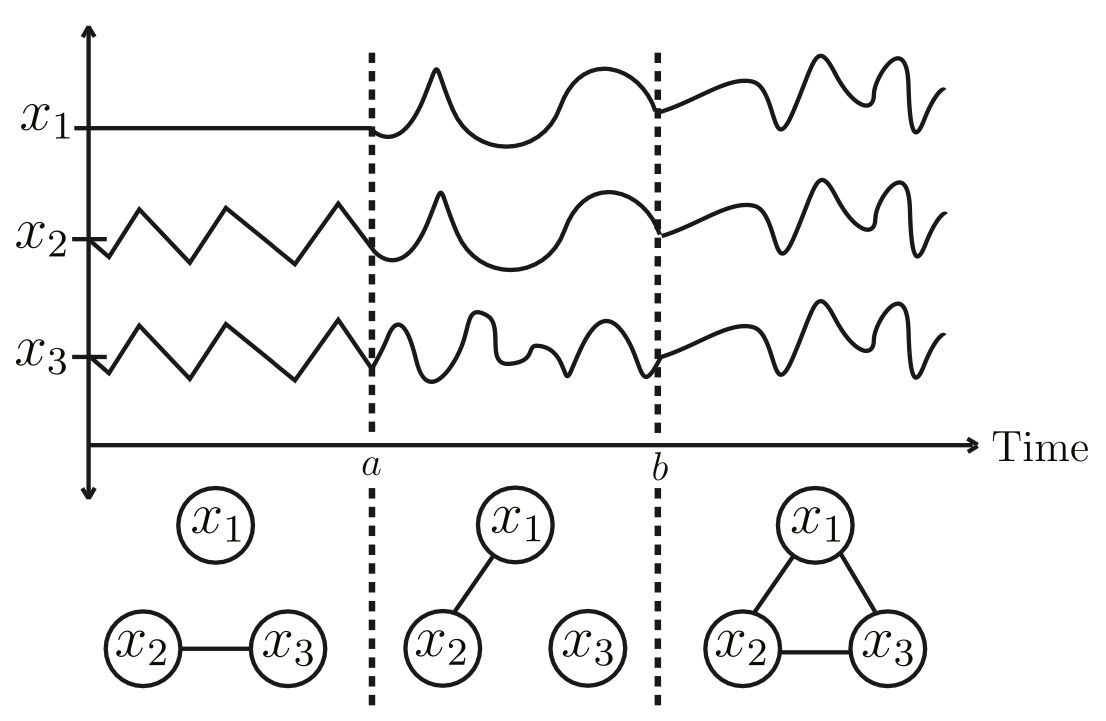
\includegraphics[width=6cm]{network_evolution}
       \caption{}
       % \source{\cite(hallac2017network)}
       \label{fig:network_evolution}
  \end{figure}
\end{frame}

\begin{frame}{Solution: Optimization on a Chain Graph (TVGL)}
    \begin{figure}
       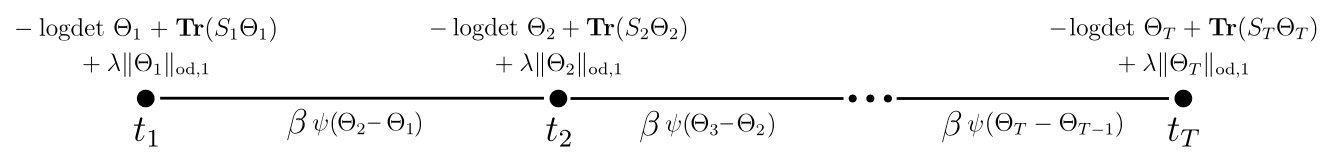
\includegraphics[width=12cm]{chain_graph.png}
       \caption{\cite{hallac2017network}}
       % \source{\cite{hallac2017network}}
       % how to choose beta?
       \label{fig:chain_graph}
  \end{figure}
    The optimization problem becomes
    \begin{align*}
        \underset{\Theta \in \mathrm{S}_{++}^{p}}{\operatorname{minimize}} \quad \sum_{i=1}^{T}-l_{i}\left(\Theta_{i}\right)+\lambda\left\|\Theta_{i}\right\|_{\mathrm{od}, 1}+\beta \sum_{i=2}^{T} \psi\left(\Theta_{i}-\Theta_{i-1}\right)
    \end{align*}
    where $\beta$ determines how strongly correlated neighboring covariance estimations should be.
    A small $\beta$ will lead to $\theta$'s which fluctuate from estimate-to-estimate, whereas large $\beta$'s lead to smoother estimates over time.
\end{frame}

\begin{frame}{Choice of $\psi$}
    \begin{itemize}
        \item $\psi$ allows to enforce different behaviors in the evolution of the network structure
        \item Expectations how the underlying network may change over time can be encoded into $\psi$
    \end{itemize}
    Options:
    \begin{itemize}
        % \item \textbf{A few edges changing at a time} - $\psi(X) = \sum_{i,1}|X_{i,j}|$
        % element-wise l1 penalte encourages neighboring graphs to be identical
        \item \textbf{Global restructuring} - $\psi(X) = \sum_j||[X]_j||_2$
        \item \textbf{Smoothly varying over time} - $\psi(X) = \sum_{i,j}X^2_{i,j}$
        % \item \textbf{Block-wise restructuring} - $\psi(X) = \sum_j\left( max_i|X_{i,j}| \right)$
        \item \textbf{Perturbed node} - $\psi(X)=\min _{V: V+V^{T}=X} \sum_{j}\left\|[V]_{j}\right\|_{2}$
    \end{itemize}
\end{frame}

\begin{frame}{Optimization Algorithm: ADMM}
	\begin{itemize}
		\item The authors use ADMM (alternating direction method of multipliers) to solve the TVGL optimization problem.
		\item ADMM is an general optimization technique that can be used on any convex optimization problem. 
		\item ADMM has a couple main advantages compared to standard gradient descent based methods: (1) Can be applied to nonsmooth functions, (2) Can be distributed across multiple independent machines
		\item To put ADMM into context, we show how it can be used to solve a generic optimization problem
	\end{itemize}
\end{frame}

\begin{frame}{Optimization Algorithm: ADMM}
\framesubtitle{General Example}
We can take the generic minimization problem
\[\underset{x}{argmin} \ f(x) \quad s.t. \ x \in \mathcal{C}\]
And separate it into two functions, $f$ and $g$, where $g$ is the indicator of $\mathcal{C}$
\[\underset{x}{argmin} \ f(x) + g(z) \quad s.t. \ x - z = 0\]
\begin{center} The variable $z$ is known as a consensus variable, and the constraint ensures final convergence between $x$ and $z$ \end{center}
\end{frame}

\begin{frame}{Optimization Algorithm: ADMM}
\framesubtitle{Proximal Operators/Proximal Gradient Descent}
The generality of the ADMM optimization technique relies on the method of proximal gradient descent. Proximal gradient descent makes use of proximal operators, defined as:
\[\operatorname{prox}_{\lambda f}(v)=\underset{x}{\operatorname{argmin}}\left(f(x)+(1 / 2 \lambda)\|x-v\|_{2}^{2}\right)\]
The ADMM iteration based update method is:
\begin{align} 
\nonumber x^{k+1} &:=\underset{x}{\operatorname{argmin}}\left(f(x)+(\rho / 2)\left\|x-z^{k}+u^{k}\right\|_{2}^{2}\right) 
\\ \nonumber z^{k+1} &:=\Pi_{C}\left(x^{k+1}+u^{k}\right) 
\\ \nonumber u^{k+1} &:=u^{k}+x^{k+1}-z^{k+1} 
\end{align}
Iterations stop when $u^{k} \xrightarrow{} u^{k+1}$ ($x-z = 0$ constraint satisfied)
\end{frame}

\begin{frame}{Optimization Algorithm: ADMM}
\framesubtitle{TVGL ADMM Application Overview}

For the TVGL, the authors introduce 3 consensus variables: $(Z_{0}, Z_{1}, Z_{2})$

\begin{enumerate}
	\item $Z_{0}$ is the consensus variable for the $\Theta_{i}$ within $|\Theta_{i}|_{od, 1}$
	\item $(Z_{1}, Z_{2})$ correspond to $(\Theta_{i}, \Theta_{i-1})$ within $\Psi(\Theta_{i} - \Theta_{i-1})$
\end{enumerate}
	
The augmented lagrangian for the TVGL then is:

\begin{align}
\nonumber \mathcal{L}_{\rho}&(\Theta, Z, U) =\sum_{i=1}^{T}-l\left(\Theta_{i}\right)+\lambda\left\|Z_{i, 0}\right\|_{\text {od, } 1}+\beta \sum_{i=2}^{T} \psi\left(Z_{i, 2}-Z_{i-1,1}\right)
\nonumber \\ &+(\rho / 2) \sum_{i=1}^{T}\left(\left\|\Theta_{i}-Z_{i, 0}+U_{i, 0}\right\|_{F}^{2}-\left\|U_{i, 0}\right\|_{F}^{2}\right)
\nonumber \\ &+(\rho / 2) \sum_{i=2}^{T}\left(\left\|\Theta_{i-1}-Z_{i-1,1}+U_{i-1,1}\right\|_{F}^{2}-\left\|U_{i-1,1}\right\|_{F}^{2}\right.
\nonumber \\ & \quad \quad \quad \quad \quad \left.+\left\|\Theta_{i}-Z_{i, 2}+U_{i, 2}\right\|_{F}^{2}-\left\|U_{i, 2}\right\|_{F}^{2}\right) \nonumber
\end{align}

\end{frame}

\begin{frame}{Optimization Algorithm: ADMM}
\framesubtitle{TVGL ADMM Application Overview}

Finally, the update procedure for the $k^{th}$ iteration in the TVGL is

\begin{align}
  
\end{align}
(a) $\Theta^{k+1}:=\underset{\Theta \in S_{++}^{p}}{\operatorname{argmin}} \mathcal{L}_{\rho}\left(\Theta, Z^{k}, U^{k}\right)$
(b) $\quad Z^{k+1}=\left[\begin{array}{c}Z_{0}^{k+1} \\ Z_{1}^{k+1} \\ Z_{2}^{k+1}\end{array}\right]:=\underset{Z_{0}, Z_{1}, Z_{2}}{\operatorname{argmin}} \mathcal{L}_{\rho}\left(\Theta^{k+1}, Z, U^{k}\right)$
(c) $U^{k+1}=\left[\begin{array}{c}U_{0}^{k+1} \\ U_{1}^{k+1} \\ U_{2}^{k+1}\end{array}\right]:=\left[\begin{array}{c}U_{0}^{k} \\ U_{1}^{k} \\ U_{2}^{k}\end{array}\right]+\left[\begin{array}{c}\Theta^{k+1}-Z_{0}^{k+1} \\ \left(\Theta_{1+1}^{k+1}, \ldots, \Theta_{T-1}^{k+1}\right)-Z_{1}^{k+1} \\ \left(\Theta_{2}^{k+1}, \ldots, \Theta_{T}^{k+1}\right)-Z_{2}^{k+1}\end{array}\right]$. 

\end{frame}

\begin{frame}{Static LASSO vs. TVGL}
\framesubtitle{Static Graphical LASSO}

  \begin{figure}
    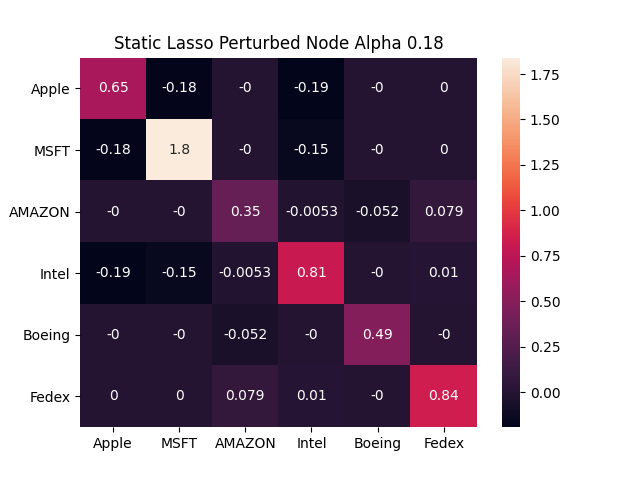
\includegraphics[width=10cm]{Static_Psi5_alpha0.18.png}
  \end{figure}

\end{frame}

\begin{frame}{Static LASSO vs. TVGL}
\framesubtitle{TVGL Perturbed Node}
\begin{center}
    \animategraphics[loop,height=8cm, width=10.5cm]{1}{PrecMatsPsi5Alpha0.18Beta13}{0}{15}
\end{center}
\end{frame}

\begin{frame}{Static LASSO vs. TVGL}
\framesubtitle{TVGL Smoothly Varying}
\begin{figure}
    \animategraphics[loop,height=8cm, width=10.5cm]{1}{PrecMatsPsi3Alpha0.18Beta13}{0}{15}
\end{figure}
\end{frame}

\begin{frame}{Importance of $\psi$}
    \begin{itemize}
        \item Choice of $\psi$ relies on knowledge about network behavior
        \item No a priori decision possible
        \item $\psi$ is fixed over time
    \end{itemize}
    We illustrate the importance of the choice of $\psi$ by comparing the author's choice of the Perturbed Node penalty function to the other two penalties
\end{frame}

\begin{frame}{Changing $\psi$}
\framesubtitle{Temporal Deviation of Precision Matrix}

\begin{figure}
  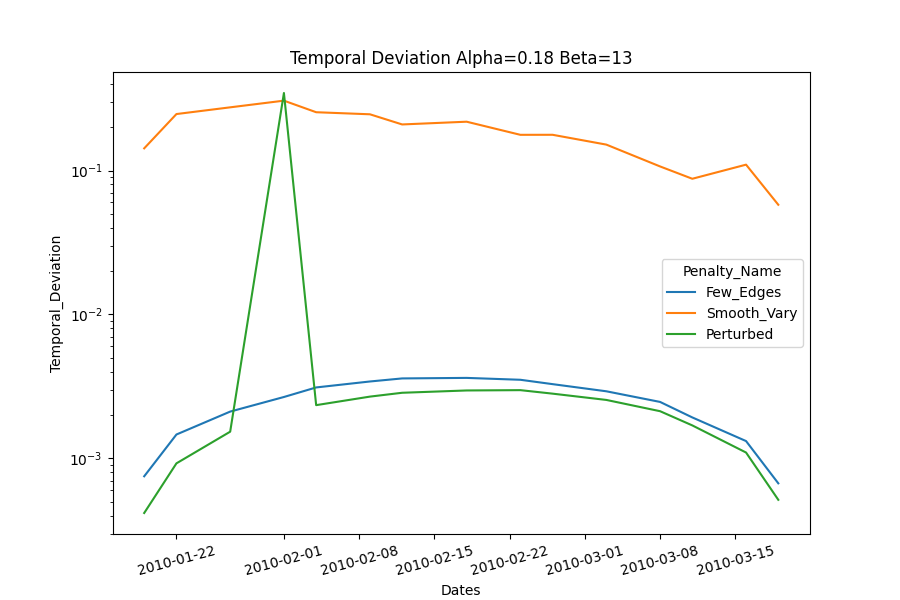
\includegraphics[width=10cm]{TemporalDevPsi1_3_5Alpha0.18Beta13.png}
  \caption{Temporal Deviation Psi Comparison}
  \label{fig:TempDev}
\end{figure}

\end{frame}

\begin{frame}{Changing $\psi$}
\framesubtitle{Temporal Deviation of Precision Matrix}

\begin{figure}
  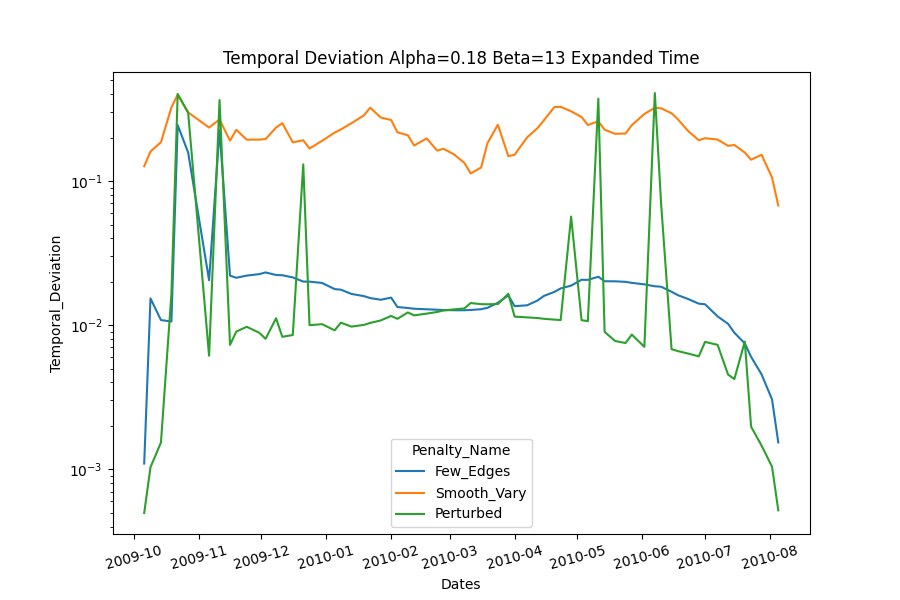
\includegraphics[width=10cm]{TemporalDevPsi1_3_5Alpha0.18Beta13TimeExpand.png}
  \caption{Temporal Deviation Psi Comparison Expanded Timespan}
  \label{fig:TempDevTimeExp}
\end{figure}

\end{frame}

\begin{frame}{Changing $\psi$}
\framesubtitle{Temporal Deviation of Precision Matrix}

\begin{figure}
  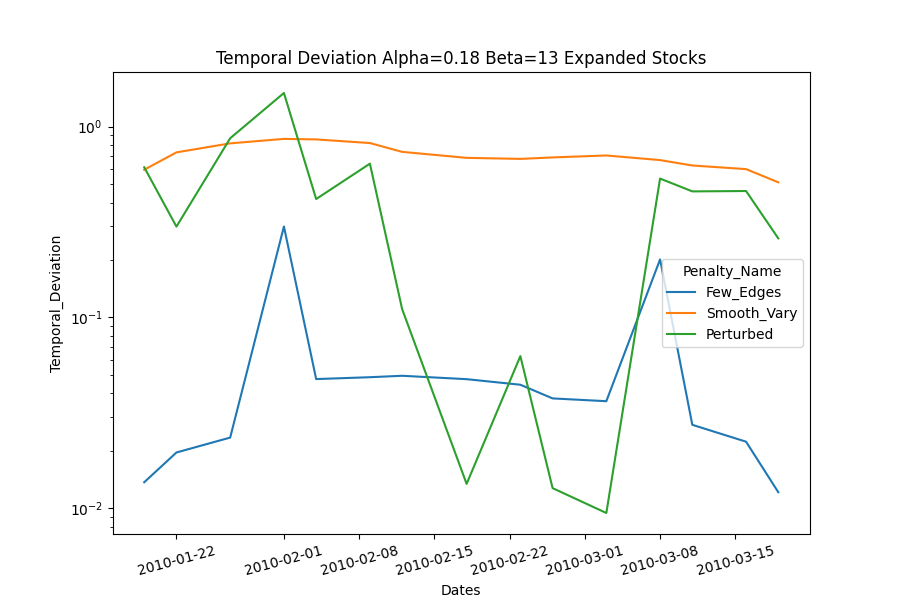
\includegraphics[width=10cm]{TemporalDevPsi1_3_5Alpha0.18Beta13StockExpand.png}
  \caption{Temporal Deviation Psi Comparison Expanded Stock Set}
  \label{fig:TempDevStockExp}
\end{figure}

\end{frame}

\begin{frame}{References}
    \nocite{*}
    \bibliographystyle{apacite}
    \bibliography{References}
\end{frame}







\end{document}